\section{Methods}
\label{sec:methods}

\subsection{VL+CT Integrator}

This is a step through of the VL+CT (Van Leer plus Constrained Transport) added too Cholla. The specific algorithm is from \citeyear[Stone \& Gardiner][]{stone_2009}.

Overall the algorithm is very similar to the Van Leer algorithm, though with significant new additions for Constrained Transport (CT). CT treats the magnetic field as surface, rather than volume, averaged quantities then updates using edge averaged EMF (Electromotive Force). By updating with EMF you automatically fulfill the divergence free condition for magnetic fields so no magnetic monopoles will appear, assuming that the initial conditions are divergence free.

\subsection*{Glossary of Symbols}

\begin{enumerate}
    \item $ \vec{U} $, Vector of conserved variables. Note that the magnetic field is the face averaged value at the $ i-1/2 $ interface whereas all the other values are volume 
    \item $ \vec{W} $, Vector of primitive variables.
    \item $ \vec{F} $, The flux vector
    \item $ x, y, \text{or} z $, Subscript to indicate which vector element is in use
    \item $ i, j, k $, Subscript indices to indicate which cell the value is in
    \item $ n $, Superscript index to indicate the time step
    \item $ \delta t $, the time step
    \item $ \delta x, \delta y, \delta z $, the size of each cell in the $x$, $y$, or $z$ direction
    \item $\rho  $, Density
    \item $p  $, Pressure
    \item $E $, Energy
    \item $v  $, Velocity
    \item $B $, Magnetic Flux Density, also called just the Magnetic Field
    \item $p_T $, Total pressure
    \item $ \mathcal{E} $, the EMF (Electromotive Force), in this application it can be used interchangeably with the electric fields. See the section on the CT fields for details
    \item $ C_{CFL} $, the CFL number, must be less than $1/2$
\end{enumerate}

\subsection{Step 1: Compute the Time Step}

The first thing we need to do is compute the time step which is done with this equation

$$
    \delta t = C_{CFL} \min \left(
        \frac{\delta x}{\mid v^n_{x,i,j,k} \mid + C^n_{f,i,j,k}},
        \frac{\delta y}{\mid v^n_{y,i,j,k} \mid + C^n_{f,i,j,k}},
        \frac{\delta z}{\mid v^n_{z,i,j,k} \mid + C^n_{f,i,j,k}}
    \right).
$$

Where $ C^n_f $ is the fast magnetosonic wave-speed computed using \emph{cell centered} values. Computing the cell centered magnetic field is done with a direct average of the face centered values. This cell centered magnetic field will be needed in the next two steps so make sure to keep it.

$$
    \begin{aligned}
        B^n_{x,i,j,k,} = \frac{1}{2} \left( B^n_{x,i+1/2,j,k} + B^n_{x,i-1/2,j,k} \right) \\
        B^n_{y,i,j,k,} = \frac{1}{2} \left( B^n_{y,i,j+1/2,k} + B^n_{y,i,j-1/2,k} \right) \\
        B^n_{z,i,j,k,} = \frac{1}{2} \left( B^n_{z,i,j,k+1/2} + B^n_{z,i,j,k-1/2} \right) \\
    \end{aligned}
$$

\subsection{Step 2: First Riemann Solve}

The next step is the solve the Riemann problem with the first order variables. This is identical to the standard Van Leer integrator for the hydrodynamic variables; the magnetic field is a bit more complicated since the magnetic field is stored as surface averages. The longitudinal field (i.e. the field that is stored at the interface itself) does not require reconstruction and can be used directly. The transverse fields (i.e. the fields parallel to the interface) are reconstructed using a straight average, which has already been done in step 1.

The magnetic fluxes that are returned by the Riemann solver are the face centered EMFs (section 5.3 of \citeyear[Stone et. al][]{stone_athena_2008}) however it's not trivial to convert them. According to the Athena source code this is the correct way to convert them into EMFs.

\emph{Note that the directions used here are relative to the internal workings of the HLLD solver. Since the HLLD solver is inherently 1D we run it three times, once for each direction. So in the case where the solver is running in the Y direction the solver's Y field is actually the Z field and the solvers Z field is actually the X field, cyclically extended for the Z direction}

\begin{table}[!ht]
    \centering
    \begin{tabular}{|l|l|l|l|}
    \hline
        HLLD solve Direction & Equation for Magnetic Flux & Eqn. as a Cross Product & EMF \\ \hline
        $ X $ & $ V_x B_y - B_x V_y $ & $  (V \times B)_z $ & $ -\varepsilon_z $ \\ \hline
        $ X $ & $ V_x B_z - B_x V_z $ & $ -(V \times B)_y $ & $  \varepsilon_y $ \\ \hline
        $ Y $ & $ V_x B_y - B_x V_y $ & $  (V \times B)_z $ & $ -\varepsilon_x $ \\ \hline
        $ Y $ & $ V_x B_z - B_x V_z $ & $ -(V \times B)_y $ & $  \varepsilon_z $ \\ \hline
        $ Z $ & $ V_x B_y - B_x V_y $ & $  (V \times B)_z $ & $ -\varepsilon_y $ \\ \hline
        $ Z $ & $ V_x B_z - B_x V_z $ & $ -(V \times B)_y $ & $  \varepsilon_x $ \\ \hline
    \end{tabular}
\end{table}

\subsection{Step 3: Compute the Constrained Transport EMF}

Now we need to calculate the CT EMF. These fields are \emph{line averaged} along each cell edge. These line averaged fields are constructed by a complicated average of the face centered EMF and their slopes which are given by the flux of the magnetic field from the Riemann solve in the previous step; i.e. the magnetic flux at a given interface is the EMF at that interface.

Technically CT uses the magnetic flux as the conservative variable and EMF to update it. However, those values only differ from the magnetic flux density (i.e. the magnetic field) and the electric field respectively by factors of unit length we can treat them as the same thing, the same way we treat density and mass as the same for the hydro fields\cite{stone_athena_2008}. As such we use the magnetic field and electric field to evolve the grid. Electric fields have the proper units to evolve the magnetic flux density, $ B $ whereas EMF has the proper units to evolve the magnetic flux.

On any face there are two non-zero electric fields; both transverse to the face. The most important thing to note is that the component that is used to calculate the field along a given edge is the component that is parallel to that edge. i.e. if the edge points along the $ z $-direction then you use the field pointing along the $ z $-direction, not the field in the $ x $ or $ y $ direction.

We also need cell centered electric fields (reference fields) for computing the slopes. This reference field can just be computed with the following cross product.

$$
    \mathcal{E}_{i,j,k}^{ref,n} = - \left( \vec{v}^{n}_{i.j.k} \times \vec{B}^{n}_{i.j.k} \right)
$$

Example for computing the CT electric field in the $ z $-direction. The other direction can be computed by just substituting out the $ z $ index with $ x $ or $ y $ and changing the derivatives appropriately, see the image in this section for more details on derivatives. The following three equations are from \citeyear[Stone \& Gardiner][]{stone_2009}, equations 22-24. In the original paper there are a few sign errors which have been fixed in the document.

$$
    \begin{aligned}
        \mathcal{E}_{z, i-1/2, j-1/2, k} = \frac{1}{4} \left(
              \mathcal{E}_{z, i-1/2, j, k}
            + \mathcal{E}_{z, i, j-1/2, k}
            + \mathcal{E}_{z, i-1/2, j-1, k}
            + \mathcal{E}_{z, i-1, j-1/2, k}\right) \\
        + \frac{\delta y}{8} \left( \left( \frac{\partial \mathcal{E}_z }{\partial y} \right)_{i-1/2, j-1/4, k} + \left(  \frac{\partial \mathcal{E}_z }{\partial y} \right)_{i-1/2, j-3/4, k} \right) \\
        + \frac{\delta x}{8} \left( \left( \frac{\partial \mathcal{E}_z }{\partial x} \right)_{i-1/4, j-1/2, k} + \left(  \frac{\partial \mathcal{E}_z }{\partial x} \right)_{i-3/4, j-1/2, k} \right)
    \end{aligned}
$$

Where the derivatives are computed using the "upwind" direction as follows.

$$
    \left( \frac{\partial \mathcal{E}_z }{\partial y} \right)_{i-1/2, j-1/4, k} =
        \begin{cases}
            \left( \frac{\partial \mathcal{E}_z }{\partial y} \right)_{i-1, j-1/4, k} & \text{for} \; v_{x, i-1/2} > 0
            \\
            \\
            \left( \frac{\partial \mathcal{E}_z }{\partial y} \right)_{i, j-1/4, k} & \text{for} \; v_{x, i-1/2} < 0
            \\
            \\
            \frac{1}{2} \left( \left( \frac{\partial \mathcal{E}_z }{\partial y} \right)_{i-1, j-1/4, k} + \left( \frac{\partial \mathcal{E}_z }{\partial y} \right)_{i, j-1/4, k} \right) & \text{otherwise}
            \\
            \\
        \end{cases}
$$

Where, for example, the derivatives are given by

$$
    \left( \frac{\partial \mathcal{E}_z }{\partial y} \right)_{i, j-1/4, k} =
    2 \left( \frac{\mathcal{E}_{z,i,j-1/2,k} - \mathcal{E}_{z,i,j,k}^{ref}}{\delta y} \right).
$$

The easiest way to see how to compute these derivatives is with the following diagrams based off of Figure 5 in \citeyear[Stone et al.][]{stone_athena_2008}. Each edge requires 4 derivatives and they are computed as differences between a reference state and an edge state.

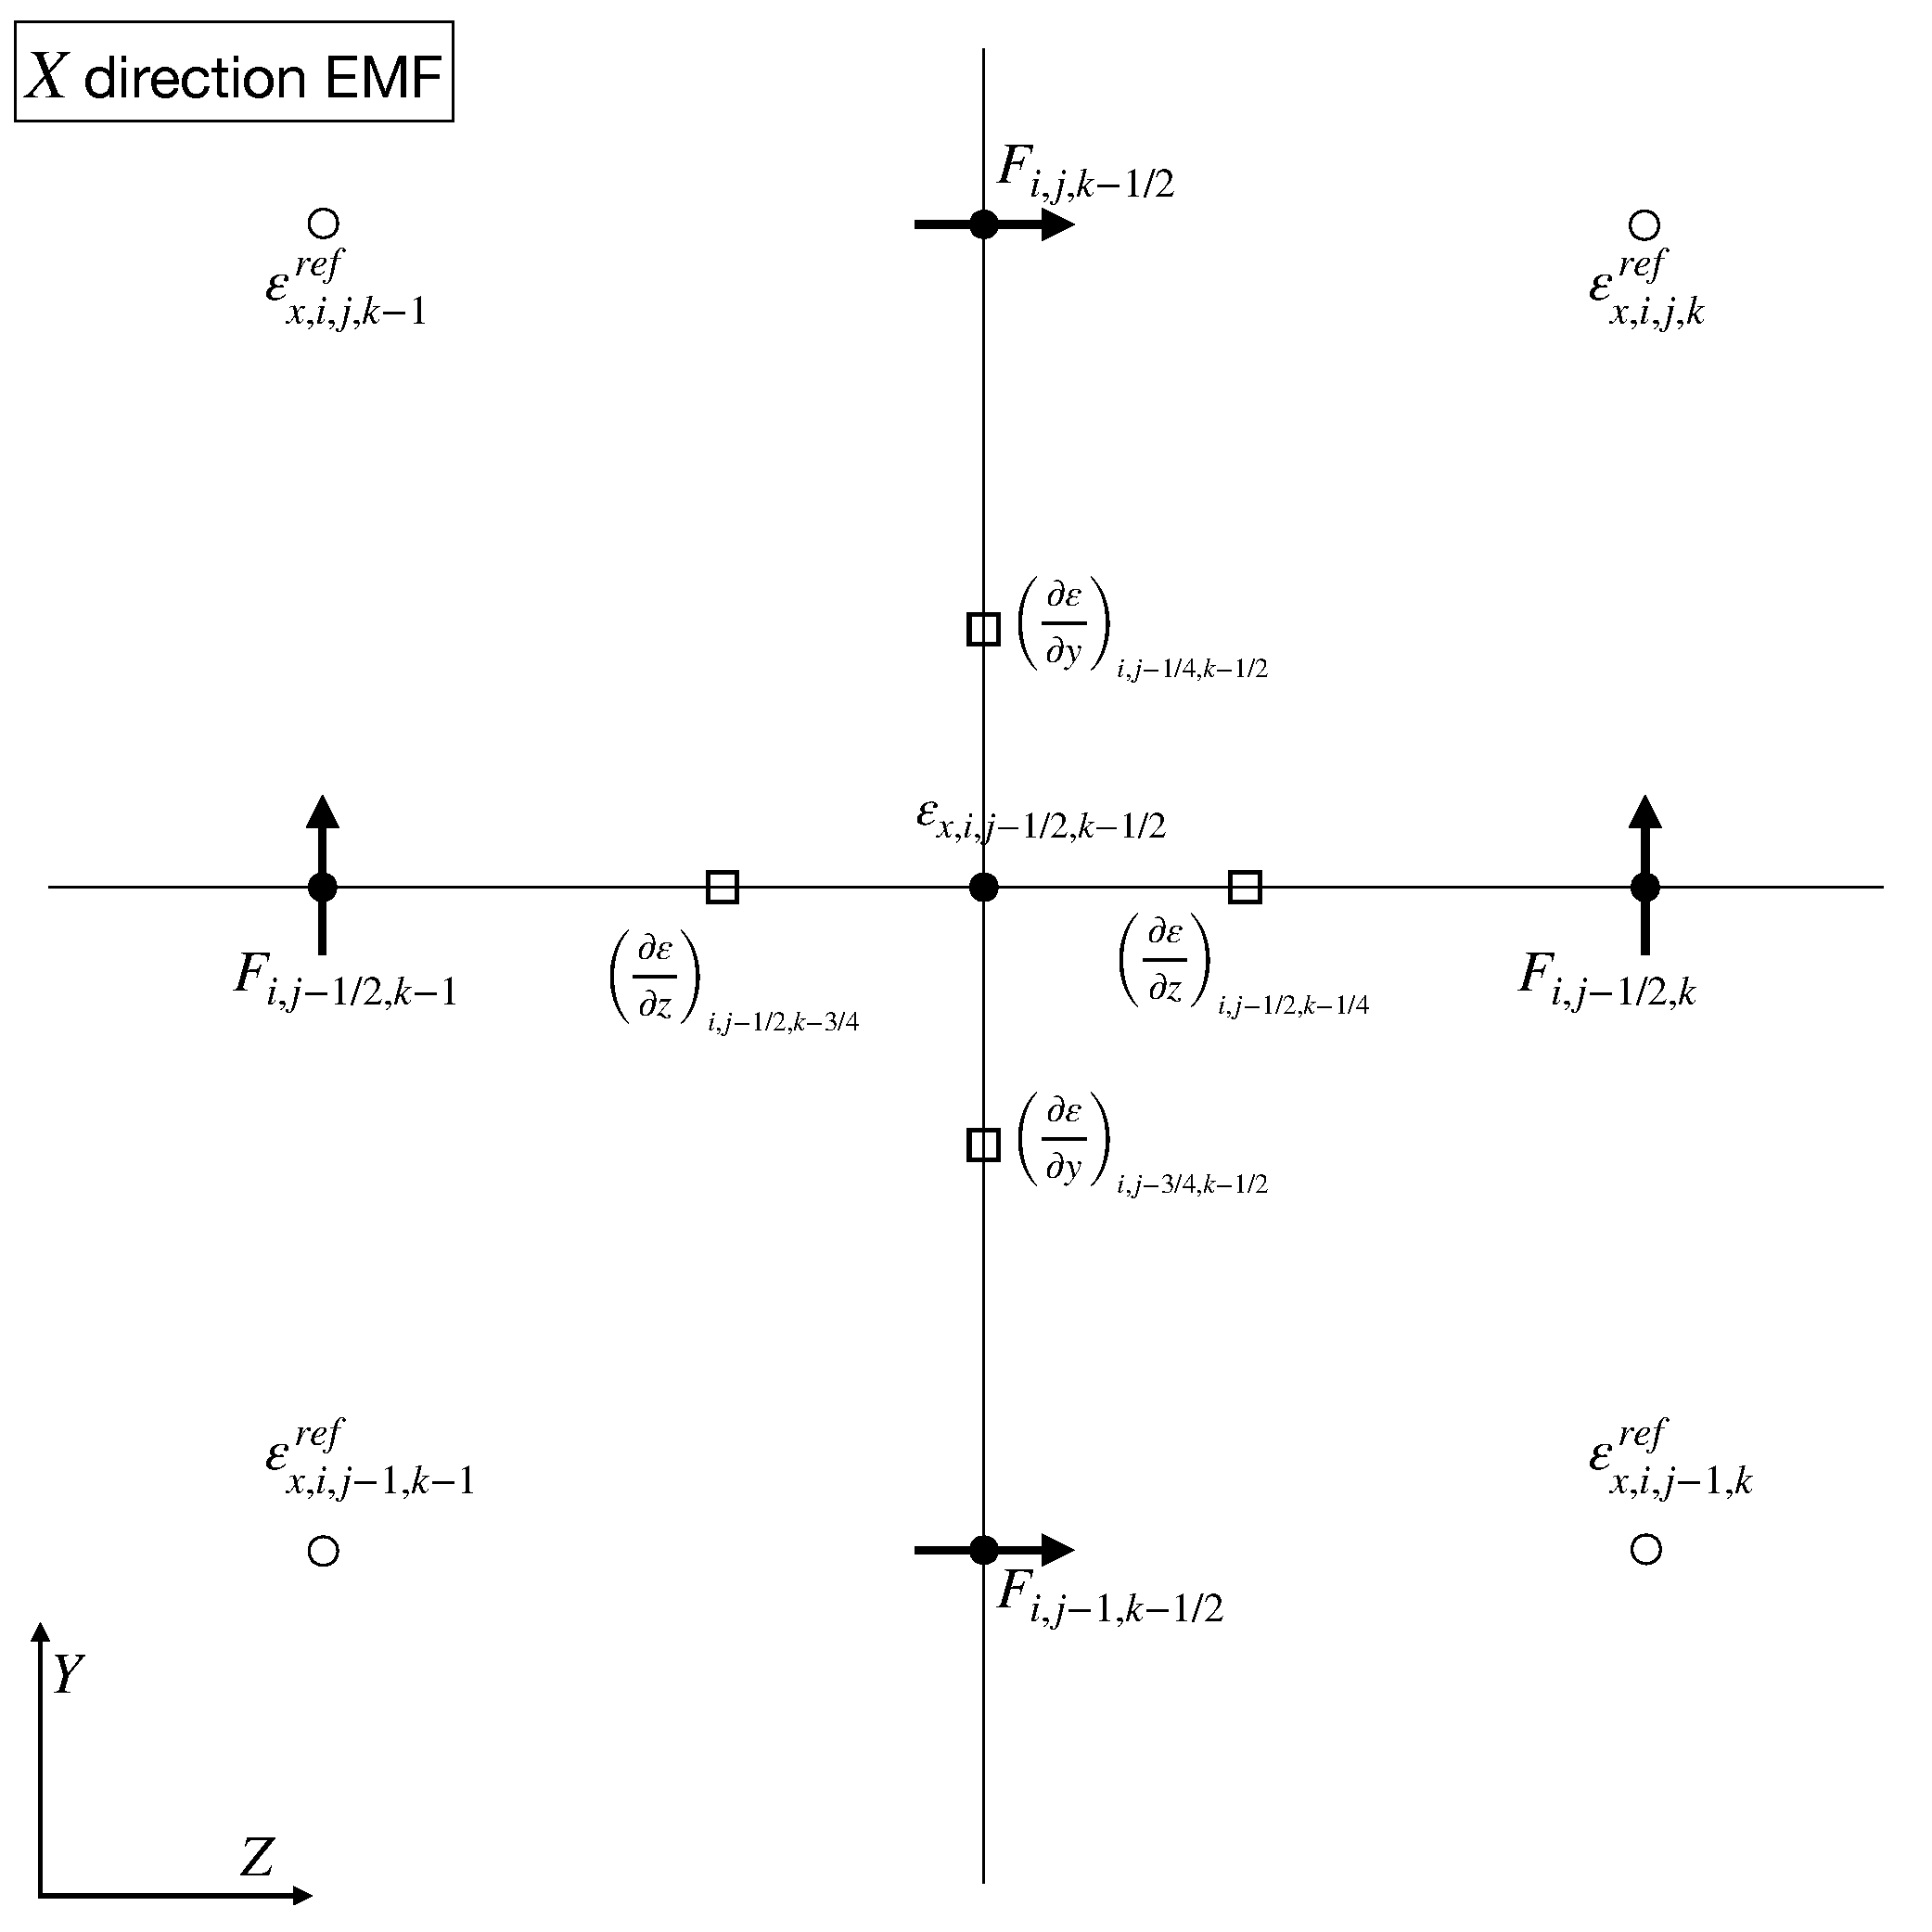
\includegraphics[scale=0.25]{Assets/2-methods/CT-edge-field-figures-X.pdf}
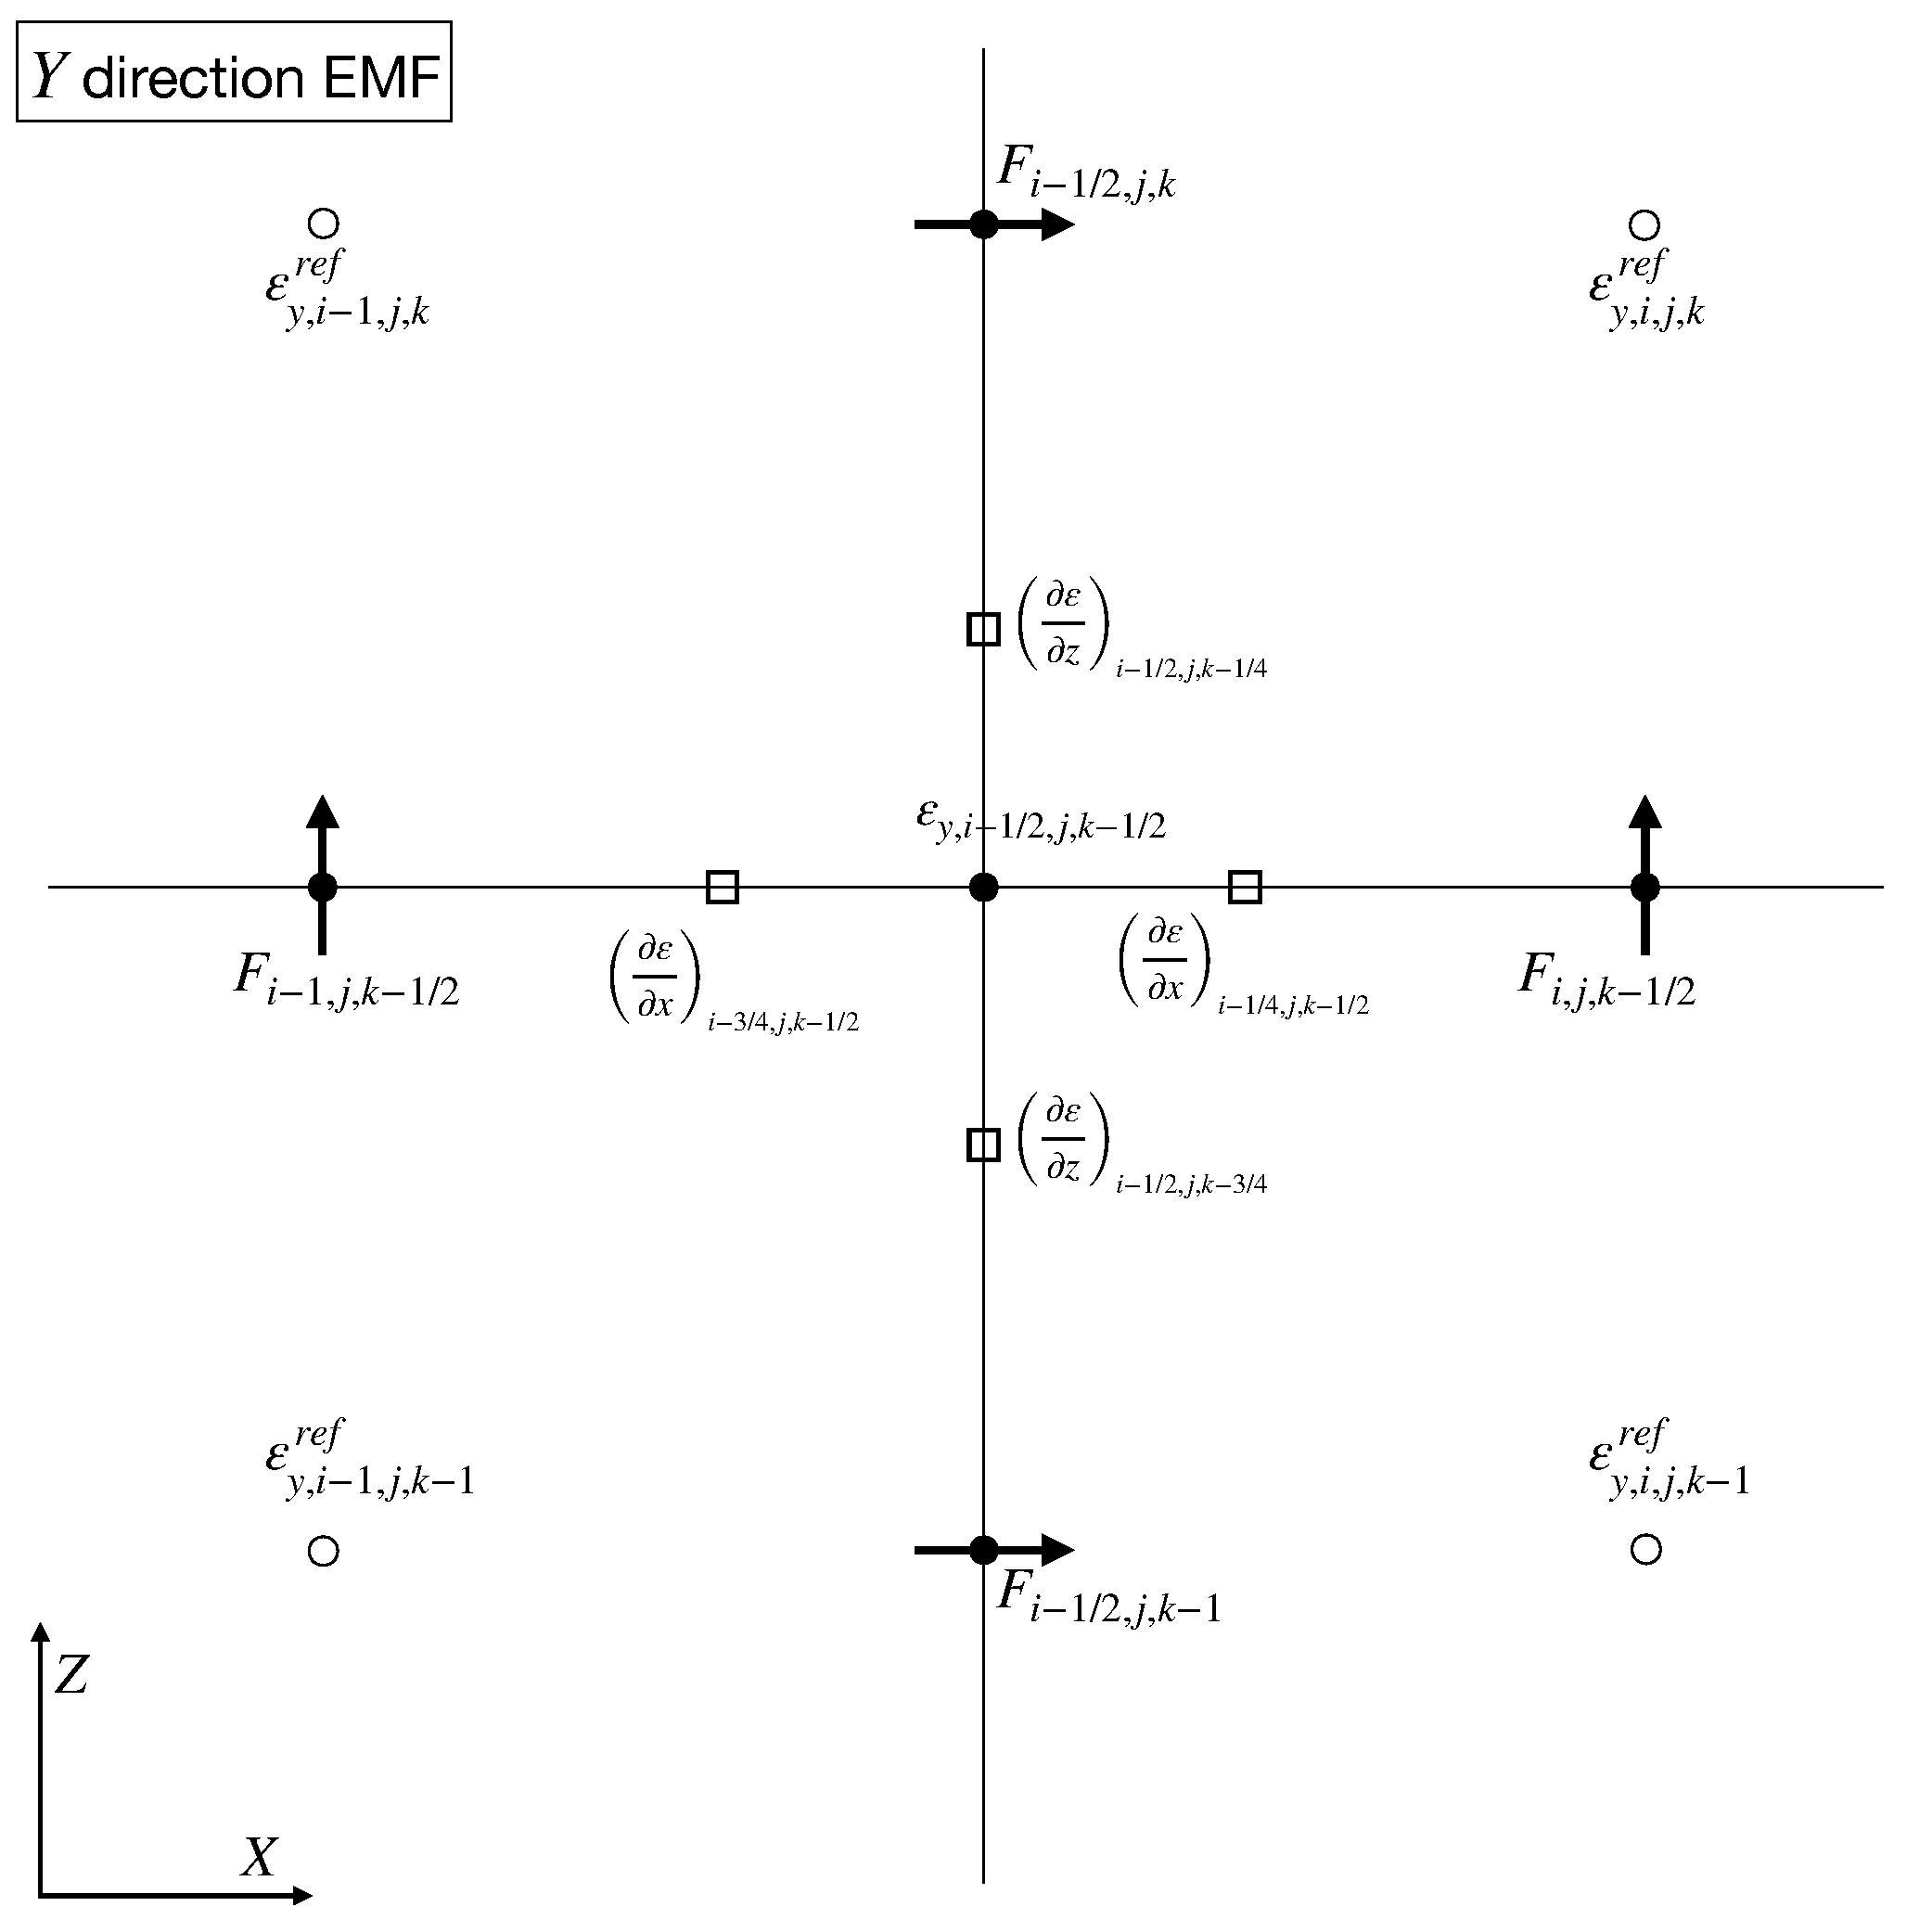
\includegraphics[scale=0.25]{Assets/2-methods/CT-edge-field-figures-Y.pdf}
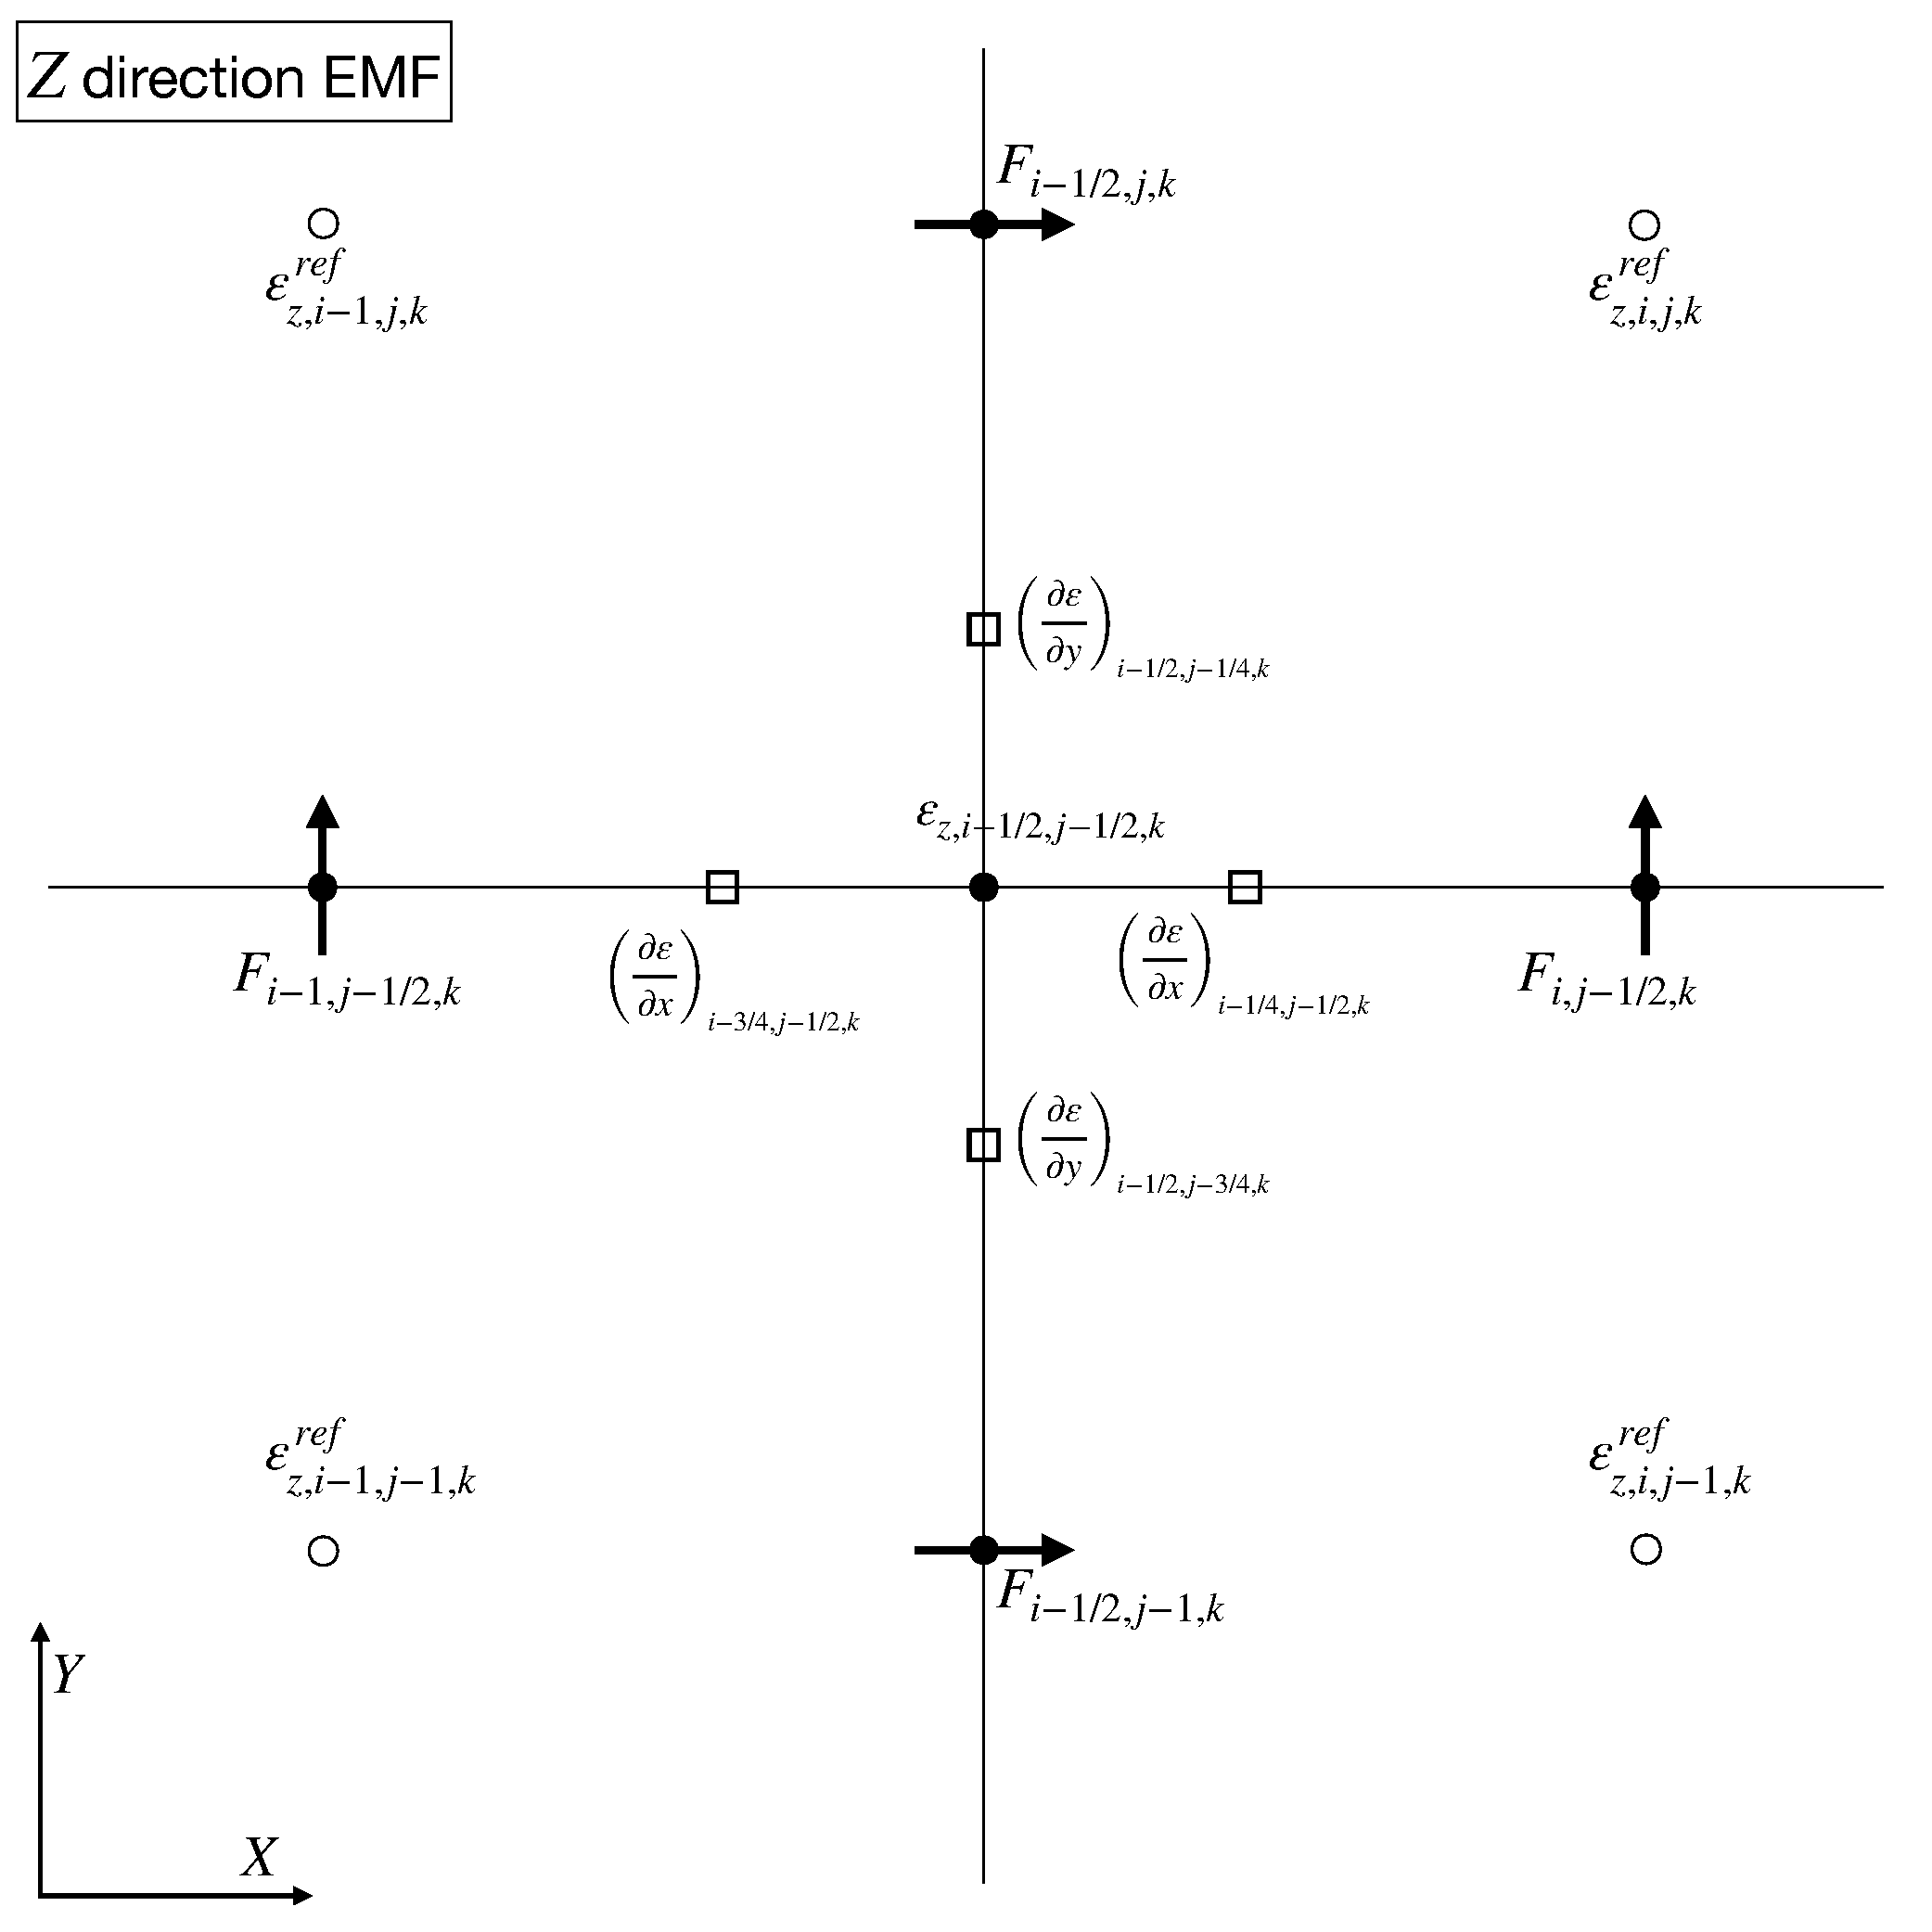
\includegraphics[scale=0.25]{Assets/2-methods/CT-edge-field-figures-Z.pdf}

\subsection{Step 4. Perform the Half Time-step Update}

Update all the hydro variables using this equation

$$
    \begin{aligned}
        \vec{U}^{n+1/2}_{i,j,k} = \vec{U}^{n}_{i,j,k}
        - \frac{\delta t}{\delta x} \left( \vec{F}^n_{x,i+1/2,j,k} - \vec{F}^n_{x,i-1/2,j,k} \right) \\
        - \frac{\delta t}{\delta y} \left( \vec{F}^n_{y,i+1/2,j,k} - \vec{F}^n_{y,i-1/2,j,k} \right) \\
        - \frac{\delta t}{\delta z} \left( \vec{F}^n_{z,i+1/2,j,k} - \vec{F}^n_{z,i-1/2,j,k} \right).
    \end{aligned}
$$

Update the magnetic field using these equations

$$
    \begin{aligned}
        B^{n+1/2}_{x,i-1/2,j,k} = B^{n}_{x,i-1/2,j,k}
        + \frac{\delta t}{\delta z} \left( \mathcal{E}^n_{y,i-1/2,j,k+1/2} - \mathcal{E}^n_{y,i-1/2,j,k-1/2} \right) \\
        - \frac{\delta t}{\delta y} \left( \mathcal{E}^n_{z,i-1/2,j+1/2,k} - \mathcal{E}^n_{z,i-1/2,j-1/2,k} \right)
    \end{aligned}
$$

$$
    \begin{aligned}
        B^{n+1/2}_{y,i,j-1/2,k} = B^{n}_{y,i,j-1/2,k}
        + \frac{\delta t}{\delta x} \left( \mathcal{E}^n_{z,i+1/2,j-1/2,k} - \mathcal{E}^n_{z,i-1/2,j-1/2,k} \right) \\
        - \frac{\delta t}{\delta z} \left( \mathcal{E}^n_{x,i,j-1/2,k+1/2} - \mathcal{E}^n_{x,i,j-1/2,k-1/2} \right)
    \end{aligned}
$$

$$
    \begin{aligned}
        B^{n+1/2}_{z,i,j,k-1/2} = B^{n}_{z,i-1/2,j,k}
        + \frac{\delta t}{\delta y} \left( \mathcal{E}^n_{x,i,j+1/2,k-1/2} - \mathcal{E}^n_{x,i,j-1/2,k-1/2} \right) \\
        - \frac{\delta t}{\delta x} \left( \mathcal{E}^n_{y,i+1/2,j,k-1/2} - \mathcal{E}^n_{y,i-1/2,j,k-1/2} \right).
    \end{aligned}
$$

\subsection{Step 5. Compute Cell Centered Magnetic Fields}

Average the values on the faces to compute the cell centered magnetic fields.
We'll need this for the second order reconstruction.

$$
    \begin{aligned}
        B^{n+1/2}_{x,i,j,k,} = \frac{1}{2} \left( B^{n+1/2}_{x,i+1/2,j,k} + B^{n+1/2}_{x,i-1/2,j,k} \right) \\
        B^{n+1/2}_{y,i,j,k,} = \frac{1}{2} \left( B^{n+1/2}_{y,i,j+1/2,k} + B^{n+1/2}_{y,i,j-1/2,k} \right) \\
        B^{n+1/2}_{z,i,j,k,} = \frac{1}{2} \left( B^{n+1/2}_{z,i,j,k+1/2} + B^{n+1/2}_{z,i,j,k-1/2} \right) \\
    \end{aligned}
$$

\subsection{Step 6. Half Time-step Second Order Reconstruction}

\textcolor{red}{This section needs updated for the characteristic step and to add PPMC}

Now we need to perform the high order reconstruction. I will show the algorithm for a second order (Piecewise Linear Method, PLM) reconstruction though any method should work. Note that at a given face only the transverse components of the electric field need to be reconstructed. The longitudinal component is already given at the face.

\begin{enumerate}
    \item Convert to primitive variables
    \item Compute the limited slopes of all the primitive variables (except the transverse magnetic field). Stone \& Gardiner 2009 suggests minmod but any TVD limiter should work fine
    \item Compute the interface states using
\end{enumerate}

    $$
        \begin{aligned}
            \vec{W}_{L, i+1/2} = \vec{W}_{i} + \frac{\delta \vec{W}_{i}^m}{2} \\
            \vec{W}_{R, i-1/2} = \vec{W}_{i} - \frac{\delta \vec{W}_{i}^m}{2} \\
        \end{aligned}
    $$

    where $ \vec{W}\_{L/R, i+1/2} $ is the state on the left or right side
    of the cell and $ \delta \vec{W}\_{i}^m $ is the monotonically limited
    slope.

\subsection{Step 7. Second Riemann Solve}

Solve the Riemann problem again with the half time step MHD interface states from step 6.

\subsection{Step 8. Compute the Constrained Transport Electric Fields}

Repeat step 3 but using the fluxes from the second Riemann solve and the half time step MHD variables.

\subsection{Step 9. Perform the Full Time-step Update}

Update all the hydro variables using the below equations. Note that this is almost identical to step 3 except we're updating the $ t = n $ state with the $ t=n+1/2 $ fluxes/CT fields instead of the $ t=n $ fluxes/CT fields.

$$
    \begin{aligned}
        \vec{U}^{n+1}_{i,j,k} = \vec{U}^{n}_{i,j,k}
        - \frac{\delta t}{\delta x} \left( \vec{F}^{n+1/2}_{x,i+1/2,j,k} - \vec{F}^{n+1/2}_{x,i-1/2,j,k} \right) \\
        - \frac{\delta t}{\delta y} \left( \vec{F}^{n+1/2}_{y,i+1/2,j,k} - \vec{F}^{n+1/2}_{y,i-1/2,j,k} \right) \\
        - \frac{\delta t}{\delta z} \left( \vec{F}^{n+1/2}_{z,i+1/2,j,k} - \vec{F}^{n+1/2}_{z,i-1/2,j,k} \right).
    \end{aligned}
$$

Update the magnetic field using these equations

$$
    \begin{aligned}
        B^{n+1}_{x,i-1/2,j,k} = B^{n}_{x,i-1/2,j,k}
        + \frac{\delta t}{\delta z} \left( \mathcal{E}^{n+1/2}_{y,i-1/2,j,k+1/2} - \mathcal{E}^{n+1/2}_{y,i-1/2,j,k-1/2} \right) \\
        - \frac{\delta t}{\delta y} \left( \mathcal{E}^{n+1/2}_{z,i-1/2,j+1/2,k} - \mathcal{E}^{n+1/2}_{z,i-1/2,j-1/2,k} \right)
    \end{aligned}
$$

$$
    \begin{aligned}
        B^{n+1}_{y,i,j-1/2,k} = B^{n}_{y,i,j-1/2,k}
        + \frac{\delta t}{\delta x} \left( \mathcal{E}^{n+1/2}_{z,i+1/2,j-1/2,k} - \mathcal{E}^{n+1/2}_{z,i-1/2,j-1/2,k} \right) \\
        - \frac{\delta t}{\delta z} \left( \mathcal{E}^{n+1/2}_{x,i,j-1/2,k+1/2} - \mathcal{E}^{n+1/2}_{x,i,j-1/2,k-1/2} \right)
    \end{aligned}
$$

$$
    \begin{aligned}
        B^{n+1}_{z,i-1/2,j,k} = B^{n}_{z,i-1/2,j,k}
        + \frac{\delta t}{\delta y} \left( \mathcal{E}^{n+1/2}_{x,i,j+1/2,k-1/2} - \mathcal{E}^{n+1/2}_{x,i,j-1/2,k-1/2} \right) \\
        - \frac{\delta t}{\delta x} \left( \mathcal{E}^{n+1/2}_{y,i+1/2,j,k-1/2} - \mathcal{E}^{n+1/2}_{y,i-1/2,j,k-1/2} \right).
    \end{aligned}
$$

\subsection{Step 10. Increment the Time by \texorpdfstring{$\delta t$}{dt}}

And that's it! Just loop this until you've reached or exceed max time and you're done!
